\chapter{Architettura hardware}
%\markboth{Introduzione}{Introduzione}
\label{cap:architettura}

In questo capitolo viene descritta in dettaglio la componentistica hardware utilizzata per l'implementazione del gioco.

\section{Unità di elaborazione}
Sia l'elaborazione dei dati trasmessi dal robot che la definizione dei comportamenti del robot in base alle logiche di gioco sono gestiti da un elaboratore esterno. Inoltre, l'elaboratore viene utilizzato dal giocatore per controllare lo stato del gioco (punteggio, tempo rimanente, \dots) e per gestirne l'avvio.

\section{Il robot}

%TODO bisogna dire che per l'interpretazione dei pacchetti in arrivo è stato fatto reversing da un vecchio progetto etc etc etc? (forse meglio metterlo in architetture sw...)

L'attore principale del gioco è il robot autonomo \emph{Spykee}, un modello commerciale della Meccano \cite{spykeeweb}, disponibile nel laboratorio di Intelligenza Artificiale e Robotica (AIRLab) del Politecnico di Milano. Questo modello è già stato utilizzato con successo in precedenti progetti nell'ambito dei Robogame\footnote{in particolare nelle varie versioni di Robowii, l'ultima delle quali è descritta in \cite{robowii}}.

Spykee si muove tramite due cingoli (con tecnica differential drive). Una telecamera montata sulla testa permette di catturare immagini compresse in formato JPEG con una risoluzione di $320 \times 240$ pixel a una frequenza di circa $20$ frame al secondo. Per comunicare con il computer che effettua il controllo, il robot crea all'accensione una rete Wi-Fi ad-hoc.

\begin{figure}[h]
\centering
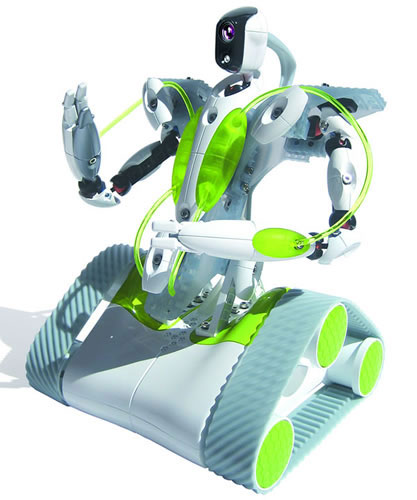
\includegraphics[scale=0.4]{images/spykee}
\caption{Il robot Spykee}
\end{figure}

\subsection*{Aggiunte hardware}
A partire da quanto già realizzato nei precedenti progetti, Spykee è stato dotato di ulteriori sensori che lo rendono adatto all'utilizzo all'interno del gioco. Tutti i componenti hardware aggiunti al robot sono controllati da un microcontrollore. A questo scopo è stata utilizzata una scheda STM32F4 Discovery Board della ST, dotata di un processore ARM Cortex M4, scelta per le sue caratteristiche: in particolare il grande numero di porte (GPIO, timer, seriali) utilizzabili.

Il firmware realizzato per controllare i vari dispositivi è stato sviluppato utilizzando il sistema operativo ChibiOS/RT\cite{chibios}. L'utilizzo di un sistema operativo per microcontrollori permette di utilizzare concetti quali thread e mutex, nonché di astrarre l'hardware sottostante, consentendo quindi una certa modularità (isolando ogni funzione in un thread indipendente) e quindi un rapido sviluppo del firmware.

La Discovery Board comunica con l'unità di elaborazione tramite un collegamento wireless di tipo Zigbee (utilizzando un modulo XBee della Digi). Il protocollo Zigbee è caratterizzato da una bassa velocità di trasmissione (comunque ampiamente sufficiente per gli scopi del progetto), ma da una buona facilità di utilizzo, specialmente in ambito embedded: viene infatti utilizzato come un collegamento seriale punto-punto tra microcontrollore e computer.

%TODO sistemare!
Le varie schede elettroniche sono state raccolte in una apposita scatola, e sono alimentate dal pacco batteria di Spykee tramite un regolatore di tensione, che permette di ridurre la tensione proveniente dalla batteria (circa $9$ V) a quella di $5$ V. Un apposito interruttore, posto a valle dell'interruttore di alimentazione di Spykee, permette di spegnere o accendere le aggiunte hardware.

\paragraph{Sonar e led} Per rilevare, e quindi evitare, eventuali ostacoli incontrati durante il movimento del robot, sono stati montati quattro sonar MaxSonar\textregistered-EZ della MaxBotix, uno per ognuno dei punti cardinali (nord, sud, ovest, est). L'aggiunta di questo tipo di dispositivi è necessaria in quanto il robot non è progettato per muoversi autonomamente, ma soltanto per ricevere comandi impartiti manualmente. 

Inoltre, Spykee è stato dotato di due strisce di LED (quattro LED gialli, quattro rossi e uno verde) che permettono di mostrare alcune informazioni relative allo stato del robot e/o del gioco nel complesso.
\begin{nota}
Sul robot sono anche presenti due led a infrarossi, che venivano utilizzati insieme a un controller Wiimote in precedenti progetti, ma che non sono di interesse per questo gioco. Le altre aggiunte hardware verranno descritte nei paragrafi successivi, essendo strettamente collegate ad altri componenti del gioco.
\end{nota}

%TODO bisogna spiegare l'interfaccia del firmware? (comandi che riceve, pinout, ...)

\section{Ostacoli attivi}
%TODO questa roba è tutta da sistemare!!!
Un problema che si è posto riguarda l'implementazione delle \emph{trappole}, gli ostacoli che modificano il comportamento del robot.

Poiché nel gioco viene già utilizzata una telecamera per poter riconoscere alcuni oggetti, inizialmente si è pensato di implementare anche le trappole utilizzando meccanismi di visione artificiale. In particolare, sono stati presi in considerazione vari tipi di marker bidimensionali, in particolare i ``Data Matrix'' e i tag della libreria ``ARToolkitPlus''\footnote{A differenza dei codici Data Matrix, che sono pensati per contenere informazioni arbitrarie, ad esempio URL oppure informazioni di spedizione, i tag ARToolkitPlus codificano solo un id, e sono pensati per applicazioni di identificazione, localizzazione, \dots (anche in presenza di distorsioni nell'immagine o altre condizioni non ottimali).}. Purtroppo, questi meccanismi hanno dato scarsi risultati in termini di velocità oppure di qualità del riconoscimento. I difetti riscontrati sono, ad esempio, un'enorme dipendenza dalle condizioni di luce, scarsi risultati in movimento, dovuti anche alla lentezza degli algoritmi (specialmente nel caso dei Data Matrix), e alle pessime condizioni delle immagini catturate. Per questi motivi, le soluzioni basate sul riconoscimento di tag mediante visione sono state scartate.

Una soluzione che ha fornito prestazioni migliori, e che è stata adottata per l'implementazione del gioco, è l'uso di tag RFID passivi a 125 KHz, che tuttavia richiede l'aggiunta di ulteriore hardware. I tag vengono correttamente riconosciuti quando il robot passa sopra di essi, con un margine di errore accettabile. Inoltre, il loro formato (tessere di plastica della dimensione di una carta di credito) li rende abbastanza comodi per l'utilizzo da parte del giocatore. Per la lettura dei tag, è stato montato sul robot un lettore (l'ID-12 della ID-Innovations), che trasmette i dati mediante un collegamento seriale a 9600 bps alla scheda di controllo presente sul robot. Una limitazione di questo specifico modello di lettore è la presenza di un'antenna interna, che ne limita pesantemente il posizionamento.

\section{Torri e fabbriche}
Le torri e le fabbriche sono costituite semplicemente da cilindri di cartoncino di colori differenti, di dimensione tali da poter essere rilevati ed abbattuti dal robot. In particolare, si è utilizzato un cilindro di colore rosso per la torre, e tre cilindri più piccoli di colore giallo per le fabbriche. 

La base dei cilindri contiene un interruttore, che risulta chiuso quando il cilindro è appoggiato a terra, e viene aperto all'abbattimento della torre. L'apertura dell'interruttore attiva un trasmettitore (del tipo di quelli utilizzati per comandare i cancelli elettrici) che invia un segnale radio a un ricevitore posto sul robot, e quindi segnala all'unità di elaborazione l'abbattimento di una torre o di una fabbrica.

Il ricevitore montato sul robot è il RX-4M-HCS prodotto dall'Aurel, ed è dotato di quattro canali separati con uscita open-drain (corrispondenti ai quattro pulsanti presenti sui corrispondenti trasmettitori, sempre della stessa marca). Pertanto, si sono impostati i relativi ingressi del microcontrollore come ingressi pull-up. Le uscite del ricevitore possono essere impostate, durante l'associazione con i trasmettitori, sia in modalità monostabile (ossia sono attive quando l'interruttore è chiuso) che in modalità bistabile (cambiano stato alla pressione dell'interruttore). Per la nostra applicazione si è scelto di utilizzare la modalità monostabile.  %TODO quest'ultimo paragrafo è da rivedere!